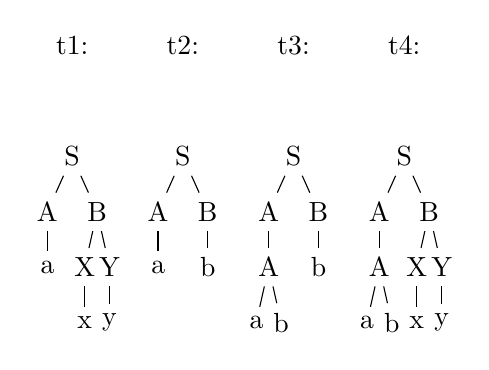
\begin{tikzpicture}
[node distance = 40 pt, sibling distance=18pt, level distance=20pt,level 2/.style={sibling distance=9pt},level 3/.style={sibling distance=9pt}]

\node (t1) {t1:}
node [ below of= t1] {S}
child {node {A} 	child {node {a}}
	}
child {node {B}	child{node {X}	child{node {x}}}
			child{node {Y}	child{node {y}}}
	}
;

\node [right of = t1] (t2) {t2:}
node [ below of= t2] {S}
child {node {A} 	child {node {a}}
	}
child {node {B}	child{node {b}}
	}
;

\node [right of = t2] (t3) {t3:}
node [ below of= t3] {S}
child {node {A} 	child {node {A}	child{node {a}}
						child{node {b}}
				}
	}
child {node {B}	child{node {b}}
	}
; 

\node [right of = t3] (t4) {t4:}
node [ below of= t4] {S}
child {node {A} 	child {node {A}	child{node {a}}
						child{node {b}}
				}
	}
child {node {B}	child{node {X}	child{node {x}}}
			child{node {Y}	child{node {y}}}
	}
;
\end{tikzpicture}